%%%%%%%%%%%%%%%%%%%%%%%%%%%%%%%%%%%%%%%%%
% Beamer Presentation
% LaTeX Template
% Version 1.0 (10/11/12)
%
% This template has been downloaded from:
% http://www.LaTeXTemplates.com
%
% License:
% CC BY-NC-SA 3.0 (http://creativecommons.org/licenses/by-nc-sa/3.0/)
%
%%%%%%%%%%%%%%%%%%%%%%%%%%%%%%%%%%%%%%%%%

%----------------------------------------------------------------------------------------
%	PACKAGES AND THEMES
%----------------------------------------------------------------------------------------

\documentclass{beamer}

\mode<presentation> {

% The Beamer class comes with a number of default slide themes
% which change the colors and layouts of slides. Below this is a list
% of all the themes, uncomment each in turn to see what they look like.

%\usetheme{default}
%\usetheme{AnnArbor}
%\usetheme{Antibes}
%\usetheme{Bergen}
%\usetheme{Berkeley}
%\usetheme{Berlin}
%\usetheme{Boadilla}
%\usetheme{CambridgeUS}
%\usetheme{Copenhagen}
%\usetheme{Darmstadt}
%\usetheme{Dresden}
%\usetheme{Frankfurt}
%\usetheme{Goettingen}
%\usetheme{Hannover}
%\usetheme{Ilmenau}
%\usetheme{JuanLesPins}
%\usetheme{Luebeck}
%\usetheme{Madrid}
%\usetheme{Malmoe}
%\usetheme{Marburg}
%\usetheme{Montpellier}
%\usetheme{PaloAlto}
\usetheme{Pittsburgh}
%\usetheme{Rochester}
%\usetheme{Singapore}
%\usetheme{Szeged}
%\usetheme{Warsaw}

% As well as themes, the Beamer class has a number of color themes
% for any slide theme. Uncomment each of these in turn to see how it
% changes the colors of your current slide theme.

%\usecolortheme{albatross}
%\usecolortheme{beaver}
%\usecolortheme{beetle}
%\usecolortheme{crane}
%\usecolortheme{dolphin}
%\usecolortheme{dove}
%\usecolortheme{fly}
%\usecolortheme{lily}
%\usecolortheme{orchid}
%\usecolortheme{rose}
%\usecolortheme{seagull}
%\usecolortheme{seahorse}
%\usecolortheme{whale}
%\usecolortheme{wolverine}

%\setbeamertemplate{footline} % To remove the footer line in all slides uncomment this line
%\setbeamertemplate{footline}[page number] % To replace the footer line in all slides with a simple slide count uncomment this line

%\setbeamertemplate{navigation symbols}{} % To remove the navigation symbols from the bottom of all slides uncomment this line
}

\usepackage{graphicx} % Allows including images
\usepackage{booktabs} % Allows the use of \toprule, \midrule and \bottomrule in 
\usepackage{amsfonts,amsmath,amssymb,graphicx,url}
\usepackage{comment}
%----------------------------------------------------------------------------------------
%	TITLE PAGE
%----------------------------------------------------------------------------------------

\title[Short title]{Orbifold Tutte Embedding } % The short title appears at the bottom of every slide, the full title is only on the title page

\author{Xuan Li} % Your name
\institute[CS@SBU] % Your institution as it will appear on the bottom of every slide, may be shorthand to save space
{
Stony Brook University \\ % Your institution for the title page
\medskip
\textit{xuanli2@cs.stonybrook.edu} % Your email address
}
\date{\today} % Date, can be changed to a custom date

\begin{document}

\begin{frame}
\titlepage % Print the title page as the first slide
\end{frame}
\begin{frame}
\footnotesize{
\begin{thebibliography}{99} % Beamer does not support BibTeX so references must be inserted manually as below
\bibitem[Aigerman, 2015]{p1} Noam Aigerman, Yaron Lipman  (2015)
\newblock Orbifold Tutte Embeddings
\newblock \emph{ACM Transactions on Graphics (TOG) - Proceedings of ACM SIGGRAPH Asia 2015, 34(6)}
\bibitem[Aigerman, 2016]{p1}
Noam Aigerman, Yaron Lipman (2016)
\newblock Hyperbolic Orbifold Tutte Embeddings
\newblock \emph{ACM Transactions on Graphics (TOG) - Proceedings of ACM SIGGRAPH Asia 2016, 35(6)}
\end{thebibliography}
}
\end{frame}

\begin{frame}
\frametitle{Overview} % Table of contents slide, comment this block out to remove it
\tableofcontents % Throughout your presentation, if you choose to use \section{} and \subsection{} commands, these will automatically be printed on this slide as an overview of your presentation
\end{frame}

%----------------------------------------------------------------------------------------
%	PRESENTATION SLIDES
%----------------------------------------------------------------------------------------

%------------------------------------------------
\section{Introduction} % Sections can be created in order to organize your presentation into discrete blocks, all sections and subsections are automatically printed in the table of contents as an overview of the talk
%------------------------------------------------
\begin{frame}
\frametitle{Introduction}
\textbf{Injective Mesh Parameterization} 
A parameterization of a surface mesh is piece-wise linear function defined by $\phi:V\rightarrow \mathbb{R}^2$. Injective means there is no overlap or flip triangle in the parameterization.\\
~\\
\textbf{Tutte Embedding}
A Tutte embedding is to place every node into the mean of its neighbors. Convex combination maps (or harmonic maps) generalize to the weighted mean. These methods are only applicable to topological disk (\textbf{target domain must be convex}) and torus.\\
~\\
\textbf{Orbifold}
Orbifold is a generation of manifold. We can use orbifold structure to apply Tutte Embedding to other type of topology. (Sphere)
\end{frame}


\section{Preliminaries} % A subsection can be created just before a set of slides with a common theme to further break down your presentation into chunks
\subsection{Orbifold}
\begin{comment}
\begin{frame}
\frametitle{Manifold}
A manifold $M$ is a topological space which can be described by a series of homomorphism charts $\phi_i: U_i\subset M \cong \tilde{U}_i \subset \mathbb{R}^n$ ($n$ is constant - locally Euclidean). Transition maps between charts should satisfy continuity conditions.
{
\centering
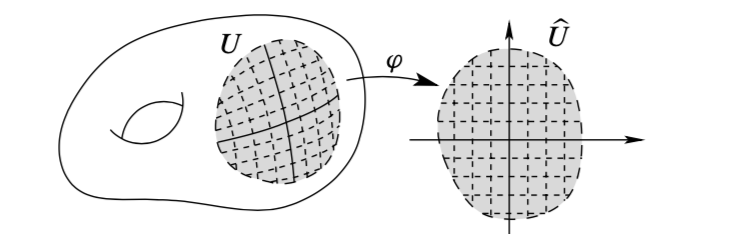
\includegraphics[width=0.5\textwidth]{images/chart}
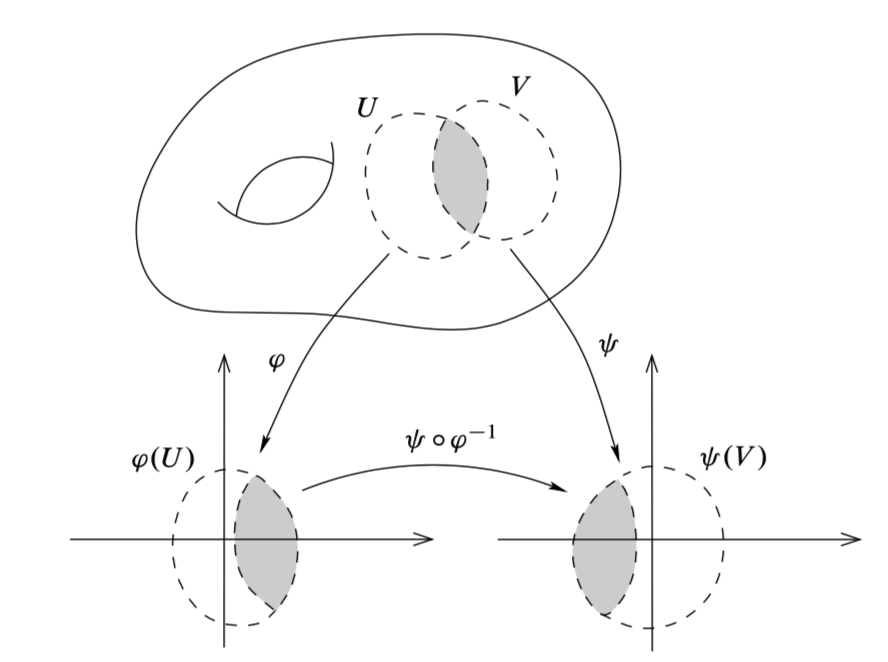
\includegraphics[width=0.5\textwidth]{images/transition}
}

\end{frame}
\end{comment}

\begin{frame}
\frametitle{Orbifold}
An orbifold(for ``orbit-manifold") is a generalization of a manifold. An orbifold $\mathit{O}$ is a topological space which has an  open cover $\{U_i\}$ closed under finite intersection.\\
~\\
\textbf{Local Chart} Each $U_i$ is associated with a finite group $\Gamma_i$ which acts on $\tilde{U}_i\subset \mathbb{R}^n$ and a homeomorphism $\phi_i: U_i \cong \tilde{U_i} / \Gamma_i$.\\
~\\
\textbf{Chart Compatibility} Whenever $U_i \subset U_j$, there is a embedding $\tilde{\phi}_{ij}: \tilde{U_i} \hookrightarrow \tilde{U_j}$ and an injective group homomorphism $f_{ij}: \Gamma_i \hookrightarrow \Gamma_j$, where $\forall \gamma \in \Gamma_i, \tilde{\phi}_{ij}(\gamma x) = f_{ij}(\gamma)\tilde{\phi}_{ij}(x)$\\
~\\
\end{frame}

\begin{comment}
\begin{frame}
\frametitle{Orbifold}
\textbf{Cone points} 
has a neighborhood homeomorphic to $\mathbb{R}^2/\mathbb{Z}_n$, $\mathbb{Z}_n$, $\mathbb{Z}_n$ is generated by rotation of $2\pi/n$.

\textbf{Mirror points} 
has a neighborhood homeomorphic to $\mathbb{R}^2/\mathbb{Z}^2$, $\mathbb{Z}^2$ acts by reflection along a line.

\textbf{Reflector corners}
has a neighborhood homeomorphic to $\mathbb{R}^2/D_n$, $\mathbb{Z}_n$, $D_n$  is the dihedral group of order 2$n$, generated by reflection about two lines meeting with angle $\pi/n$.

\end{frame}
\end{comment}


\begin{frame}
\frametitle{Examples}
Quotient space by a finite group can be treated as a tiled space by some basic tile.

\textbf{Euclidean Orbifold} An orbifold whose associated groups consist of Euclidean isometries.\\
\textbf{Hyperbolic Orbifold} An orbifold whose associated groups consist of hypobolic isometries (we mainly discuss Poincare disk model).
\begin{figure}
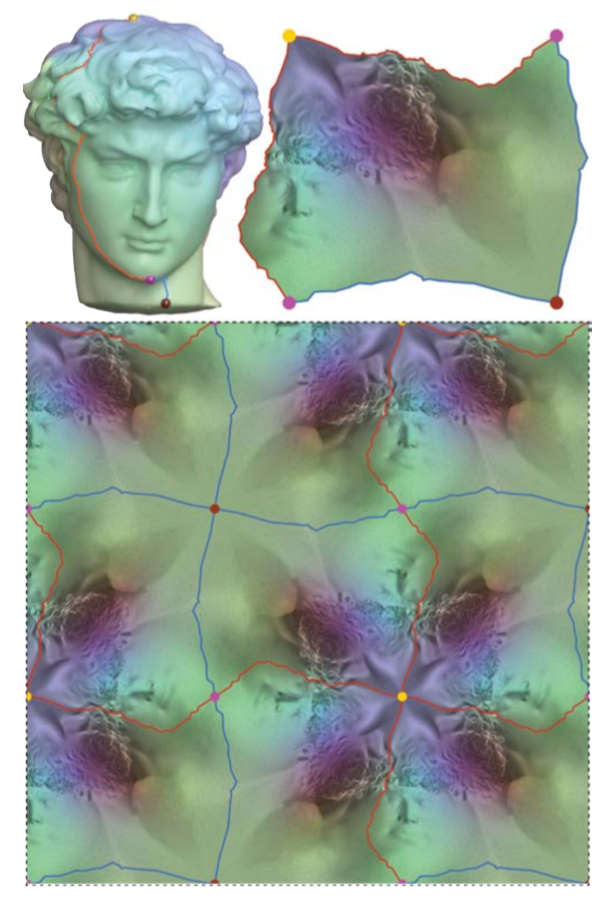
\includegraphics[width=0.3\textwidth]{images/euclidean-orbifold.png}
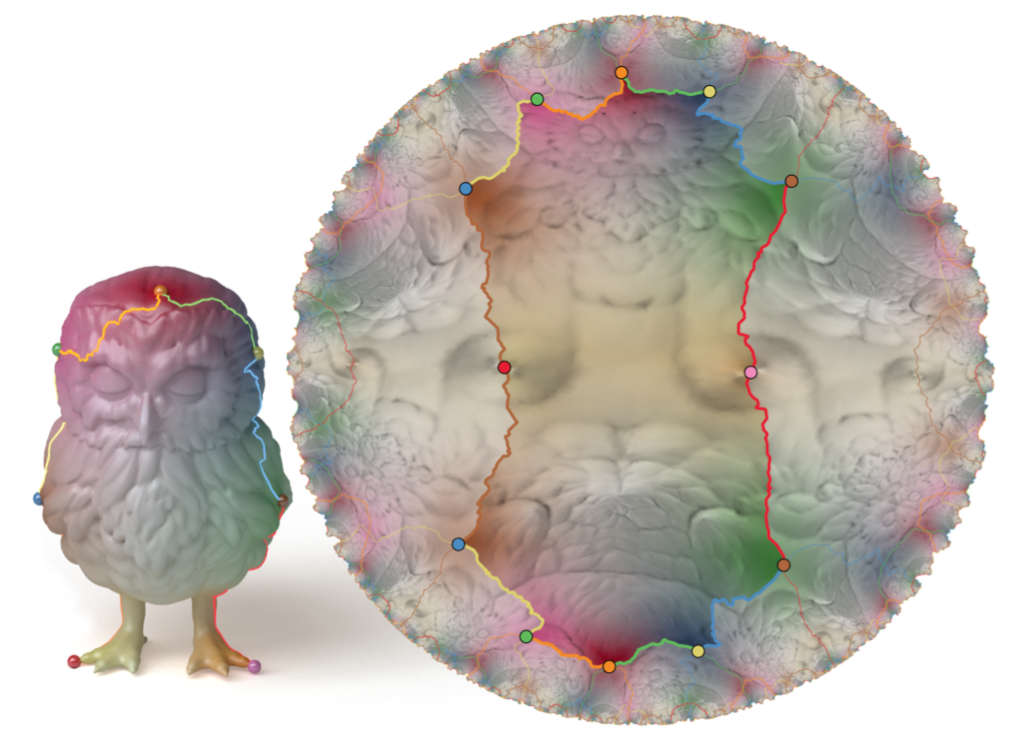
\includegraphics[width=0.5\textwidth]{images/hyperbolic-orbifold.png}
\end{figure}
\end{frame}

\begin{frame}
\frametitle{Sphere-type Orbifolds}
Orbifolds with sphere-type underlying topology. One observation: Only have cone points.\\
~\\
\textbf{Classification}\\
Define $\delta_i = 2\pi - \Theta_i.$\\
~\\ 
Euclidean sphere-type orbifold: $\sum_i \delta_i = 2\pi \chi(\mathit{O}) = 4\pi$\\
$\{\frac{\pi}{2}, \pi, \frac{\pi}{2}\}, \{\frac{2\pi}{3}, \frac{2\pi}{3}, \frac{2\pi}{3}\}, \{\pi, \frac{2\pi}{3}, \frac{\pi}{3}\}, \{\pi, \pi, \pi, \pi\}$\\
~\\
Hyperbolic sphere-type orbifold: $\sum_i \delta_i > 2\pi \chi(\mathit{O}) = 4\pi$\\
Let $\delta_i = \pi, \#cones > 4$
\end{frame}



\subsection{Tutte Embedding}
\begin{frame}
\frametitle{Convex Combination Maps}
Denote $M = (V, H, F)$ an oriented triangular disk-type mesh. $\Phi: V\rightarrow \mathbb{R}^2$ is its parameterization. And $W: H\rightarrow \mathbb{R}^+$ is a weight function on halfedges. A convex combination map satisfies:
$$ \sum_{j\in N_i} w_{ij}(\Phi_i - \Phi_j) = 0, \forall v_i \in Int(M)$$

\textbf{Tutte Embedding:} $w_{ij} = 1$

\textbf{Harmonic Map:} $w_{ij} = \frac{\cot \alpha_{ij} + \cot \beta_{ij}}{2}$ 

\begin{figure}
\centering
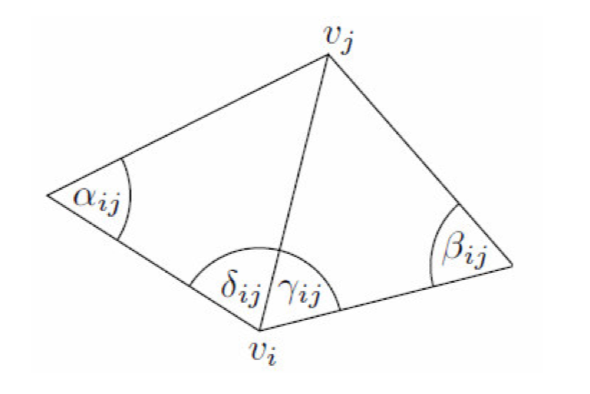
\includegraphics[width = 0.3\textwidth]{images/harmonic}
\end{figure}
Uniquely defined by boundary value, and injective.
\end{frame}



\section{Approach}
\subsection{Euclidean Orbifold Tutte Embedding}
\begin{frame}
\frametitle{Euclidean Orbifold Tutte Embedding}
1. Slice: Choose some cone points in $\bar{M}$ and cut the mesh to a disk $M$.\\
~\\
2. Chart Map: Compute a parameterization of $M$ s.t. it becomes a base domain of some orbifold. It's injective.\\
~\\
3. Orbifold Map: induce a bijective map from $\bar{M}$ to the orbifold.
\end{frame}

\begin{frame}
\frametitle{Euclidean Orbifold Tutte Embedding}
$\bar{M}$ is a spherical surface mesh. Assume $\{\bar{v}_i\}_{i = 1}^I$ is the set of cone points we choose. \\
~\\
We can only "see" the orbifold by a \textbf{chart}:
Find a path $\bar{v}_1\rightarrow \bar{v}_2\rightarrow ...\rightarrow \bar{v}_I $. Cut the mesh to disk topology $M$ along this slice to get a chart.\\
~\\
Each vertex $\bar{v}_i$ on the slice will be split into two vertices $v_i$ and $v_{i'}$, they are \textbf{equivalent} under a rotation $R_{ii'}$ of some cone point.\\
~\\
Our goal: get $\bar{\Phi}: \bar{M}\rightarrow \mathit{O}$ from $\Phi: M\rightarrow \mathbb{R}^2$
\end{frame}

\begin{frame}
\frametitle{Sphere-type Euclidean Orbifolds}
\begin{figure}
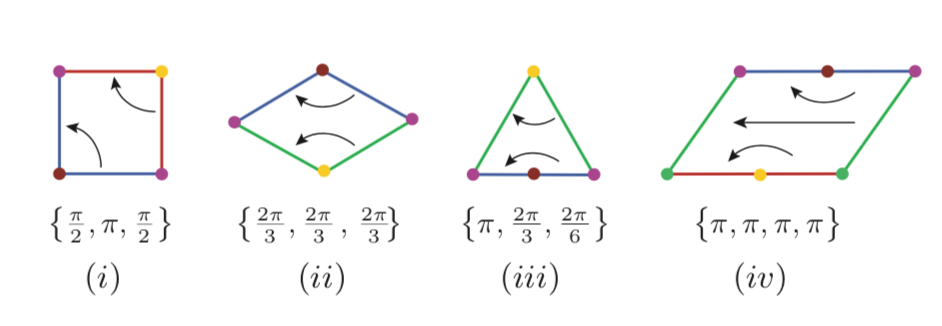
\includegraphics[width=\textwidth]{images/orbifolds}
\end{figure}
\end{frame}

\begin{frame}
\frametitle{Linear System for Euclidean Orbifold}
The singularities becomes $\{v_1, v_2, ... v_J\}$. Assign them prescribed coordinates $\{\Phi_i^C\}_{i=1}^{J}$\\
~\\
For inner vertex $v_i$:
$$\sum_{j\in N_i}(\Phi_i - \Phi_j) = 0$$
For each pair of boundary vertex $v_i$ and $v_{i'}$:
\begin{figure}
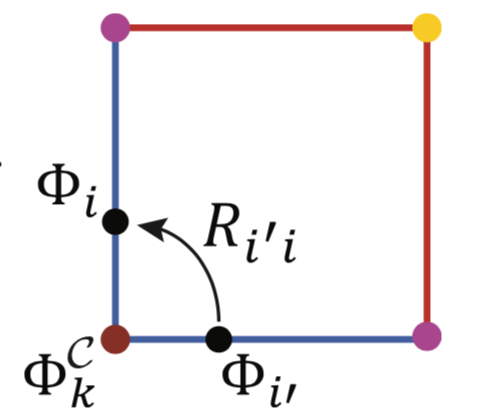
\includegraphics[width=0.2\textwidth]{images/linear-system}
\end{figure}
$$\sum_{j\in N_i}w_{ij}(\Phi_i - \Phi_j) + \sum_{j\in N_{i'}}w_{i'j}R_{i'i}(\Phi_i' - \Phi_j) = 0 $$
$$R_{i'i}(\Phi_{i'} - \Phi_k^C) - (\Phi_i - \Phi_k^C)= 0$$
\end{frame}

\begin{frame}
\frametitle{Orbifold Map}
Construct $\bar{\Phi}:\bar{M}$ as follows:
$$\bar{\Phi}(\bar{v}_i) = [\Phi(v_i)]$$

This map is invariant of the choice of slice:
\begin{figure}
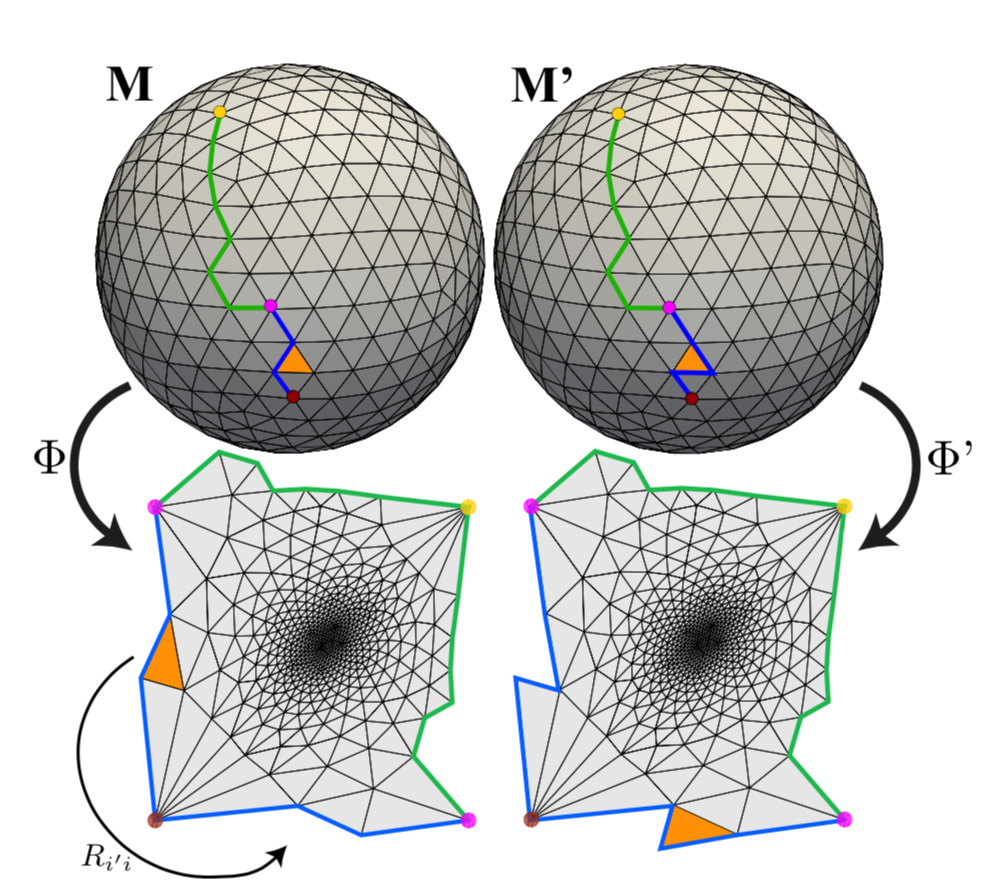
\includegraphics[width = 0.5\textwidth]{images/invariant}
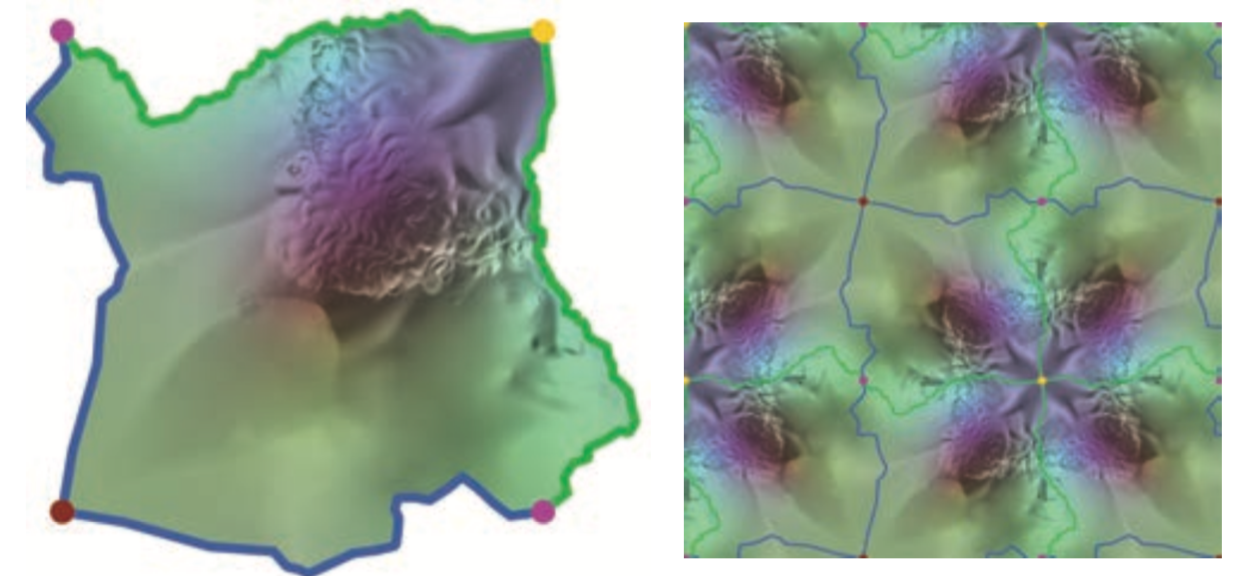
\includegraphics[width = 0.5\textwidth]{images/tiling}
\end{figure}
\end{frame}

\begin{frame}
\frametitle{Results}
\begin{figure}
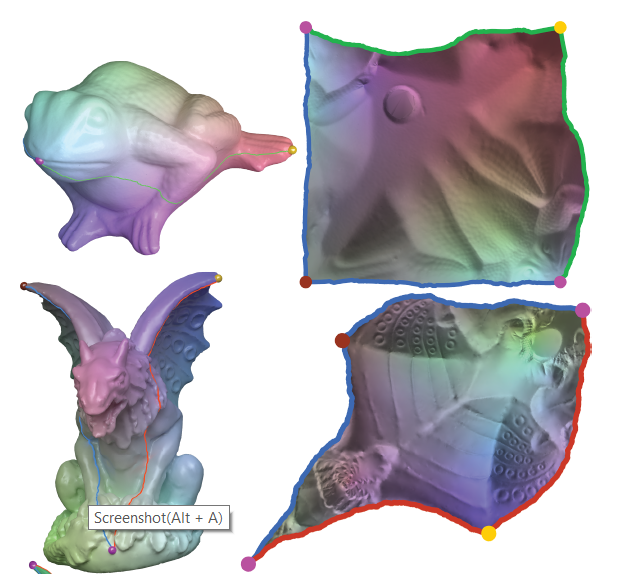
\includegraphics[width=0.5\textwidth]{images/euclidean-results1}
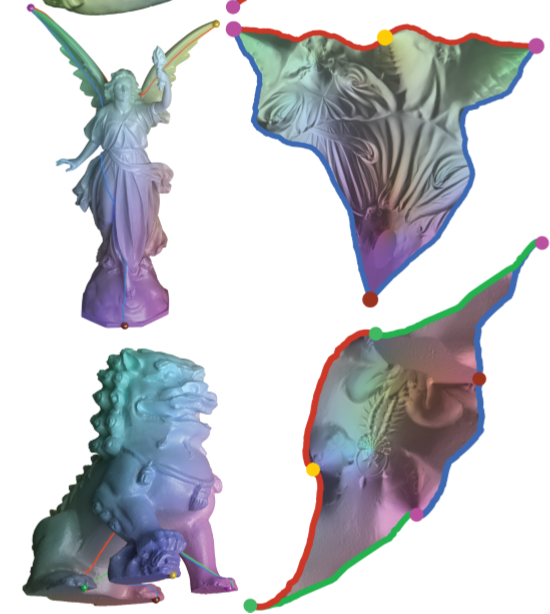
\includegraphics[width=0.5\textwidth]{images/euclidean-results2}
\end{figure}
\end{frame}
\begin{comment}
\begin{frame}
\frametitle{Properties}
\begin{theorem}
The linear system has an unique solution.
\end{theorem}
\begin{theorem}
$\Phi:M\rightarrow \mathbb{R}^2$ is globally injective. And it defines a unique bijective map 
$\bar{\Phi}:\bar{M}\rightarrow \mathit{O}$
\end{theorem}
\end{frame}



\begin{frame}
\frametitle{Conformality}
Let $w_{ij} = w_{ji}$.

\textbf{Sphere-type orbifold with 3 cone points}:

The solution of linear system is a critical point of $$E_D(\Phi) = \int_{M}|\nabla \Phi|^2$$. 

Under boundary conditions $$\Phi_k = \Phi_k^C$$
$$R_{i'i}(\Phi_{i'} - \Phi_k^C) - (\Phi_i - \Phi_k^C)= 0$$

The solution is a globally minimizer of the conformal energy
$$E_C(\Phi) = E_D(\Phi) - Area(\Phi)$$
\end{frame}

\begin{frame}
\frametitle{Conformality}
\begin{figure}
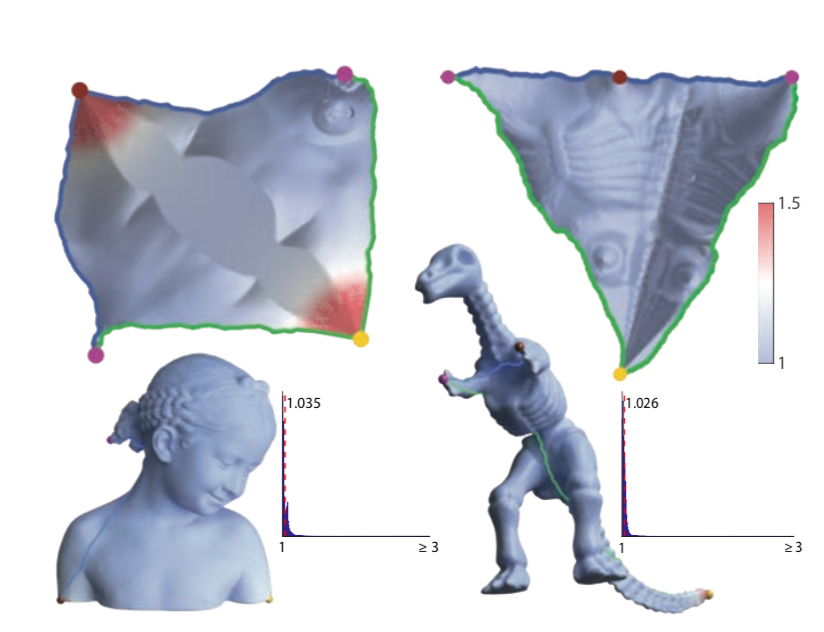
\includegraphics[width=0.8\textwidth]{images/conformal1}
\end{figure}
\end{frame}

\begin{frame}
\frametitle{Conformality}

\textbf{Sphere-type orbifold with 4 cone points}:
Minimize an global affine transformation additionally: 
\begin{equation}
\begin{split}
&\min_L E_C(L\Phi)\\
&s.t. ||L||^2_F = 1
\end{split}
\end{equation}
\begin{figure}
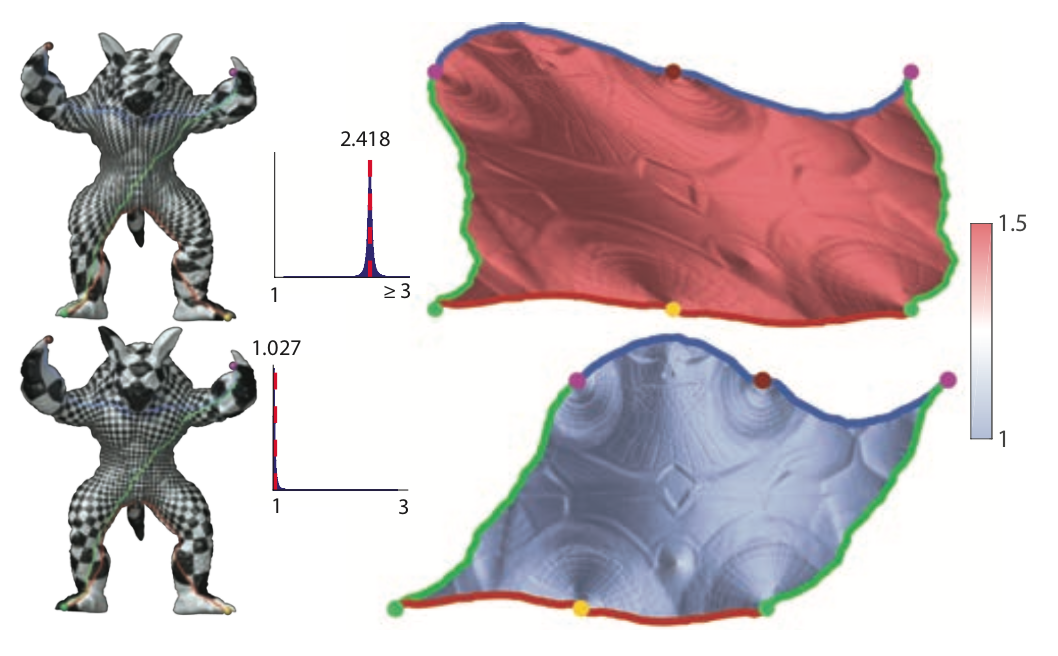
\includegraphics[width=0.7\textwidth]{images/conformal2}
\end{figure}
\end{frame}
\end{comment}


\subsection{Hyperbolic Orbifold Tutte Embedding}

\begin{frame}
\frametitle{Hyperbolic Convex Combination Map}
Non-linear! 

Assume $w_{ij} = w_{ji} > 0$.

Minimize $$ E(\Phi) = \frac{1}{2}\sum_{(i,j)\in E} = w_{ij}d(\Phi_i,\Phi_j)^2$$

$d(\Phi_i,\Phi_j)$ - geodesic distance
\end{frame}

\begin{frame}
\frametitle{Poincare Disk Model}
Hyperbolic metric:
$$ ds^2 = \frac{4|dz|^2}{(1 - |z|^2)^2}$$
Geodesic curves:
\begin{figure}
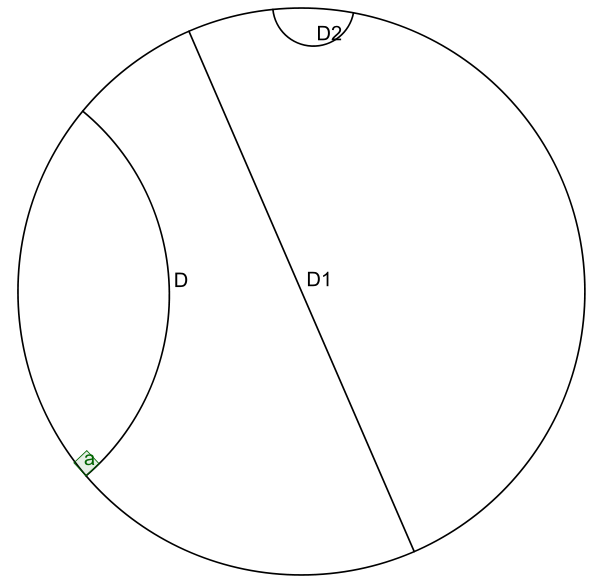
\includegraphics[width=0.5\textwidth]{images/geodesic}
\end{figure}
\end{frame}

\begin{frame}
Geodesic distance:
$$d(z, w) = \arccos(1 + 2\frac{|z - w|^2}{(1 - |z|^2)(1 - |w|^2)})$$
Isometries: Mobius transformations ($D^2\rightarrow D^2$)
$$m(z) = e^{i\theta}\frac{z - p_0}{1 - \bar{p_0}z}$$
Determined by two  points.
\end{frame}


\begin{frame}
\frametitle{Sphere-type Hyperbolic Orbifolds}
\textbf{Classification}\\
Define $\delta_i = 2\pi - \Theta_i.$\\
~\\ 
Hyperbolic sphere-type orbifold: $\sum_i \delta_i > 2\pi \chi(\mathit{O}) = 4\pi$\\
Let $\delta_i = \pi, \#cones > 4$

\begin{figure}
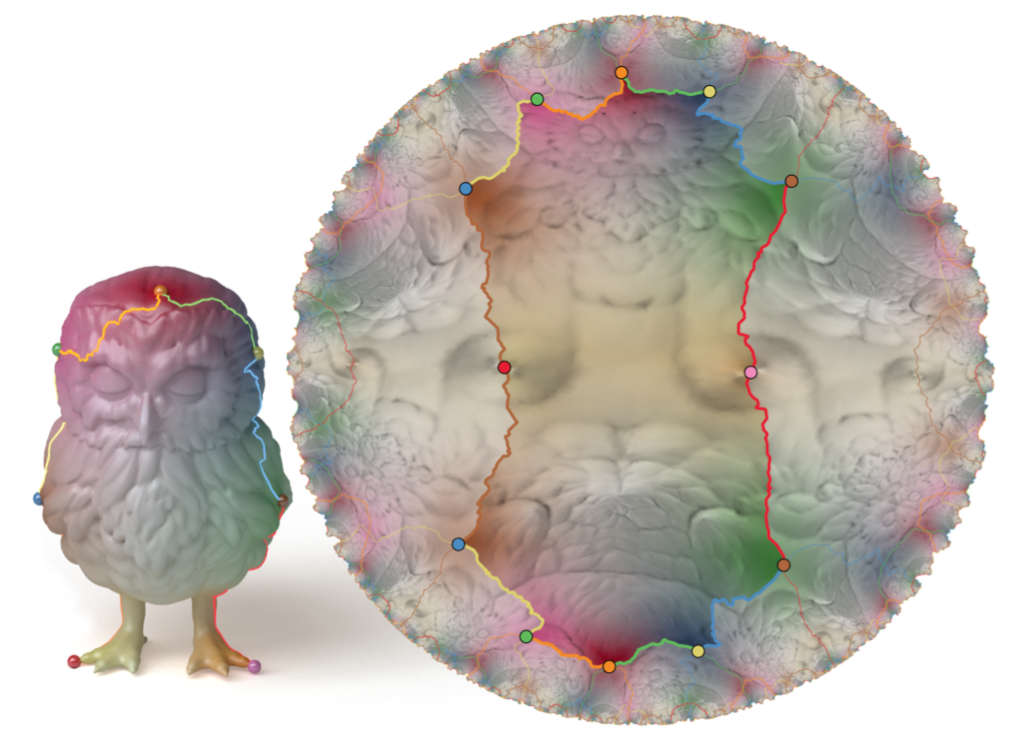
\includegraphics[width=0.5\textwidth]{images/hyperbolic-orbifold.png}
\end{figure}
\end{frame}

\begin{frame}
\frametitle{Hyperbolic Orbifold Tutte Embedding}
1. Slice: Choose some cone points in $\bar{M}$ and cut the mesh to a disk $M$.\\
~\\
2. Chart Map: Compute a parameterization of $M$ s.t. it becomes a base domain of some orbifold. It's injective.\\
~\\
3. Orbifold Map: induce a bijective map from $\bar{M}$ to the orbifold.
\end{frame}

\begin{frame}
\frametitle{Optimization}
\begin{figure}
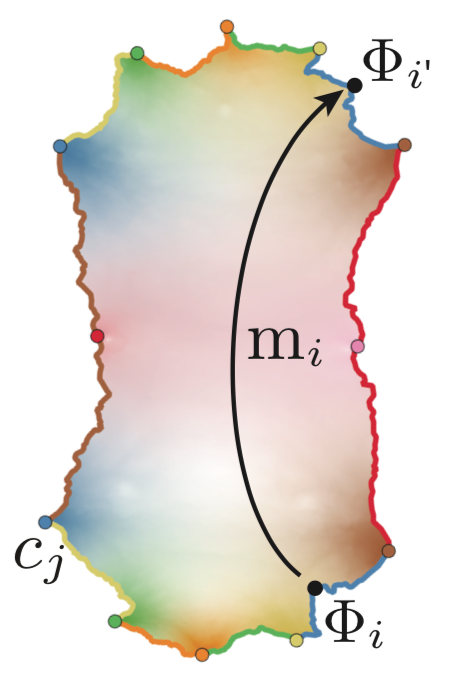
\includegraphics[width=0.3\textwidth]{images/optimize-hyperbolic}
\end{figure}
\begin{equation}
\begin{split}
&\min E(\Phi)\\
s.t. \ \  & \Phi_j = c_j,\ \ \  \hfill j\in cones\\
&\Phi_{i'} = m_i(\Phi_i),\ \ \  \hfill(i, i')\ equivalent.
\end{split}
\nonumber
\end{equation}
\end{frame}

\begin{frame}
\frametitle{Reformulate Gradient}
Insert $\Phi_{i'} = m_i(\Phi_i)$ into the energy expression.
\begin{equation}
\nonumber
\nabla_{\Phi_i} E = \sum_{j\in N_i}\nabla_{\Phi_i}w_{ij}d(\Phi_i, \Phi_j)^2 + \sum_{j\in N_{i'}}\nabla_{\Phi_i}w_{i'j}d(\Phi_i, m_i^{-1}(\Phi_j))^2
\end{equation}

Multiple gradients pointwise by $(1 - |\Phi|^2)^2 / 4$ - hyperbolic length on the disk.

Solve by first-order optimization algorithms (e.g. LBFGS)
\end{frame}

\begin{frame}
\frametitle{Properties}
\textbf{Injective chart map.} $\Phi: M\rightarrow D^2$ is injective.

\textbf{Bijective orbifold map.}
$\bar{\Phi}(\bar{v}_i) = [\Phi(v_i)]$ is bijective from $\bar{M}$ to $\mathit{O}$.
This map is invariant of the choice of slice, too.


\end{frame}

\begin{frame}
\frametitle{Results}
$k = 7$ with $\Theta_i = \pi$:
\begin{figure}
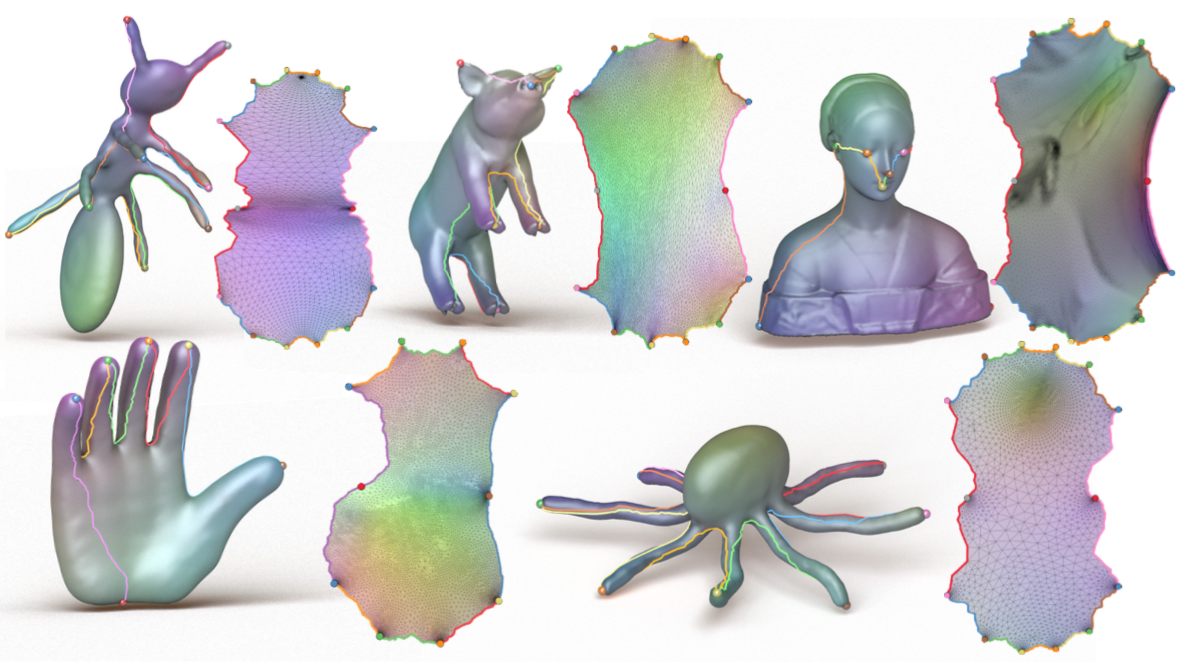
\includegraphics[width = \textwidth]{images/hyperbolic-result}
\end{figure}
\end{frame}
%------------------------------------------------



%------------------------------------------------

\begin{frame}
\Huge{\centerline{The End}}
\end{frame}

%----------------------------------------------------------------------------------------

\end{document}